\documentclass[a4paper,12pt,oneside]{book}
\usepackage[utf8]{inputenc}
\title{}
\author{Rachel Morris}
\date{\today}

\usepackage{rachwidgets}
\usepackage{fancyhdr}
\usepackage{lastpage}
\usepackage{boxedminipage}
\usepackage{fancyvrb}

\newcommand{\laClass}{CS 250\ }
\newcommand{\laSemester}{Fall 2017\ }
\newcommand{\laLab}{Lab 9: Polymorphism\ }

\pagestyle{fancy}
\fancyhf{}
\lhead{\laClass}
\chead{\laSemester}
\rhead{\laLab}
\rfoot{\thepage\ of \pageref{LastPage}}
\lfoot{By Rachel Morris, \footnotesize last updated \today}

\renewcommand{\headrulewidth}{2pt}
\renewcommand{\footrulewidth}{1pt}

\begin{document}

    \chapter*{\laLab} \stepcounter{chapter}

        \section{Information}
            \paragraph{ Topics: } Polymorphism
            \paragraph{ Turn in: } All source files (.cpp and .hpp).
            \paragraph{ Starter files: } Download on GitHub or D2L.

% ----------------------------------------------------------------------
% ----------------------------------------------------------------------
% ----------------------------------------------------------------------

\renewcommand*\DTstylecomment{\rmfamily\color{green}\textsc}

\begin{framed}
\dirtree{%
.1 Lab 09 - Polymorphism/.
.2 lab9\_main{.}cpp
    \dots{} \begin{minipage}[t]{5cm} Contains main() \end{minipage}.
.2 lab9\_game{.}hpp
    \dots{} \begin{minipage}[t]{5cm} Contains game code \end{minipage}.
.2 lab9\_Character{.}hpp
    \dots{} \begin{minipage}[t]{5cm} Character family of classes \end{minipage}.
.2 lab9\_Character{.}cpp
    \dots{} \begin{minipage}[t]{5cm} Functions for Character family functions \end{minipage}.
.2 CodeBlocks Project/
    \dots{} \begin{minipage}[t]{7cm}
        Code::Blocks project here
    \end{minipage}.
.2 Makefile/
    \dots{} \begin{minipage}[t]{7cm}
        Makefile here
    \end{minipage}.
.2 VS2015 Project/
    \dots{} \begin{minipage}[t]{7cm}
        Visual Studio 2015 project here
    \end{minipage}.
}
\end{framed}

This program does not have any tests associated with it; you will have to
manually test it by playing the game, or write your own tests.

    \tableofcontents

% ----------------------------------------------------------------------
% ----------------------------------------------------------------------
% ----------------------------------------------------------------------

    \newpage{}

    \section{Class declarations}

    First, you will add class declarations in the \texttt{lab9\_Character.hpp}
    file. This file will contain all members of the Character family of classes.

    \subsection{ICharacter interface class}

    The ICharacter class is the interface class, which will contain
    the< common functionality between all Character classes. This class
    will also contain one \textit{pure virtual function}: GetChoice().
    This function is pure virtual because each subclass will be
    \textit{required} to implement their own version of this function.

    Build the ICharacter class based on this UML diagram:

    \begin{center}
        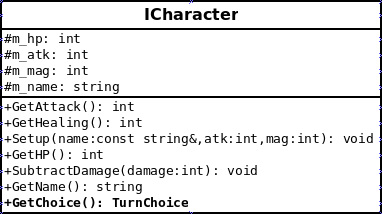
\includegraphics[height=7cm]{images/lab9-icharacter.png}
    \end{center}

    \begin{hint}{Key}
        The top section contains the member variables. The \# symbol
        means that these are \textbf{protected}.

        The bottom section are the member functions. The + symbol
        means that these are \textbf{public}.

        The function that is bold, \textbf{GetChoice()}, is a pure
        virtual function.
        To make it virtual, put the keyword \textbf{virtual}
        at the beginning of the function signature, and to make it
        pure-virtual, put \textbf{= 0} at the end of the signature.
        \begin{verbatim}
        virtual TurnChoice GetChoice() = 0;
        \end{verbatim}
    \end{hint}

    \subsection{NPC class}

    Declare the NPC class as per the diagram. The GetChoice function
    should also be marked as \textbf{virtual}, but it won't be pure-virtual,
    so don't include the \textbf{= 0} at the end.
    
    \begin{center}
        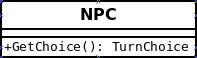
\includegraphics{images/lab9-npc.png}
    \end{center}

    \subsection{Player class}

    Declare the Player class as per the diagram. The GetChoice function
    should also be marked as \textbf{virtual}, but it won't be pure-virtual,
    so don't include the \textbf{= 0} at the end.
    
    \begin{center}
        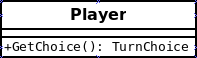
\includegraphics{images/lab9-player.png}
    \end{center}


    \newpage{}
    
    \section{Function definitions}

    Now in the .cpp file you will implement the functions.

    \subsection{ICharacter::GetAttack}

\begin{lstlisting}[style=code]
int ICharacter::GetAttack()
{
    return rand() % m_atk;
}
\end{lstlisting}

    \subsection{ICharacter::GetHealing}

\begin{lstlisting}[style=code]
int ICharacter::GetHealing()
{
    int healing = rand() % m_mag;
    m_hp += healing;

    if ( m_hp > 100 )
    {
        m_hp = 100;
    }

    return healing;
}
\end{lstlisting}

    \subsection{ICharacter::GetHP}

\begin{lstlisting}[style=code]
int ICharacter::GetHP()
{
    return m_hp;
}
\end{lstlisting}

    \subsection{ICharacter::GetName}

\begin{lstlisting}[style=code]
string ICharacter::GetName()
{
    return m_name;
}
\end{lstlisting}

    \subsection{ICharacter::Setup}

\begin{lstlisting}[style=code]
void ICharacter::Setup( const string& name, int atk, int mag )
{
    m_name = name;
    m_atk = atk;
    m_mag = mag;
    m_hp = 100;
}
\end{lstlisting}

    \subsection{ICharacter::SubtractDamage}

\begin{lstlisting}[style=code]
void ICharacter::SubtractDamage( int damage )
{
    m_hp -= damage;
}
\end{lstlisting}

    \subsection{NPC::GetChoice}

\begin{lstlisting}[style=code]
TurnChoice NPC::GetChoice()
{
    return TurnChoice( rand() % 2 );
}
\end{lstlisting}

    \subsection{Player::GetChoice}

\begin{lstlisting}[style=code]
TurnChoice Player::GetChoice()
{
    int choice;
    cout << "Select your choice: ";
    cin >> choice;
    cout << endl;
    return TurnChoice( choice );
}
\end{lstlisting}




    \newpage{}


    \section{The game}
    
    Back in \texttt{lab9\_game.hpp}, uncomment out the code in the
    \texttt{Game()} function. Afterward, take note of the following
    parts of the code:

\begin{lstlisting}[style=code]
Player player;
player.Setup( "Player", 10, 10 );

NPC npc;
npc.Setup( "Enemy", 5, 5 );

ICharacter* ptrPlayers[2];
ptrPlayers[0] = &player;
ptrPlayers[1] = &npc;
\end{lstlisting}

Here, Iv'e declared a Player object and an NPC object, as well
as an array of ICharacter pointers. Both the Player and the NPC can
be treated as ICharacter objects to use their common interface. The
game itself doesn't care which class it is, just that the functions
of ICharacter are used.

~\\~\\
Later on in the game, it reduces duplicate code by using a for-loop
to execute the same code for each player:

\begin{lstlisting}[style=code]
for ( int i = 0; i < 2; i++ )
{
    TurnChoice choice = ptrPlayers[i]->GetChoice();
\end{lstlisting}

This would be much more managable if we were going to keep building on
this program and adding more characters.
Conversely, if we had almost-duplicate code with only slight differences
back-to-back, the more characters we add, the more cluttered our code would get.

This is why we write generic \textbf{interface} classes, and then write
more specialized child classes to handle specific functionality.
In the implementation, we cut down on duplicate code, and in the design,
we spend more time thinking about how to keep the interface and the
specialized classes organized and clean.


\newpage
\subsection{Example output}

When running the game, it should look like this:

\begin{lstlisting}[style=output]
ROUND 3
Your HP: 98	Enemy HP: 92

0. Attack
1. Heal
Select your choice: 0

* Player attacks Enemy for 6 damage!
* Enemy attacks Player for 4 damage!

Press a key to continue...
\end{lstlisting}








    \newpage
    \section{Appendix A: Starter code}

\subsection*{lab9\_main.cpp}

\begin{lstlisting}[style=code]
#include <iostream>
#include <cstdlib>
using namespace std;

#include "lab9_game.hpp"

int main()
{
    Game();

    return 0;
}
\end{lstlisting}

\subsection*{lab9\_game.cpp}

\begin{lstlisting}[style=code]
#ifndef _GAME
#define _GAME

#include "lab9_Character.hpp"

void ClearScreen()
{
    #if defined(WIN32) || defined(_WIN32) || defined(__WIN32) && !defined(__CYGWIN__)
        system( "cls" );
    #else
        system( "clear" );
    #endif
}

void DrawSeparator( int length )
{
    cout << endl;
    for ( int i = 0; i < length; i++ )
    {
        cout << "-";
    }
    cout << endl;
}

void DisplayMenu( int round, int playerHP, int enemyHP )
{
    ClearScreen();
    cout << "ROUND " << round << endl;
    cout << "Your HP: " << playerHP << "\tEnemy HP: " << enemyHP << endl << endl;
    cout << "0. Attack" << endl;
    cout << "1. Heal" << endl;
}

void Game()
{
//    Player player;
//    player.Setup( "Player", 10, 10 );
//
//    NPC npc;
//    npc.Setup( "Enemy", 5, 5 );
//
//    ICharacter* ptrPlayers[2];
//    ptrPlayers[0] = &player;
//    ptrPlayers[1] = &npc;
//
//    int round = 1;
//
//    while ( ptrPlayers[0]->GetHP() > 0 && ptrPlayers[1]->GetHP() > 0 )
//    {
//        DisplayMenu( round, ptrPlayers[0]->GetHP(), ptrPlayers[1]->GetHP() );
//
//        for ( int i = 0; i < 2; i++ )
//        {
//            TurnChoice choice = ptrPlayers[i]->GetChoice();
//
//            int otherPlayer;
//            if ( i == 0 )   { otherPlayer = 1; }
//            else            { otherPlayer = 0; }
//
//            if ( choice == ATTACK )
//            {
//                int damage = ptrPlayers[i]->GetAttack();
//
//                cout    << "* " << ptrPlayers[i]->GetName() << " attacks "
//                        << ptrPlayers[ otherPlayer ]->GetName() << " for "
//                        << damage << " damage!" << endl;
//
//                ptrPlayers[ otherPlayer ]->SubtractDamage( damage );
//            }
//            else if ( choice == HEAL )
//            {
//                int health = ptrPlayers[i]->GetHealing();
//
//                cout    << "* " << ptrPlayers[i]->GetName() << " heals themself for "
//                        << health << " HP!" << endl;
//            }
//        }
//
//        cout << endl;
//
//        round++;
//
//        cout << "Press a key to continue..." << endl;
//        cin.ignore();
//        cin.get();
//    }
//
//    for ( int i = 0; i < 2; i++ )
//    {
//        if ( ptrPlayers[i]->GetHP() <= 0 )
//        {
//            cout << ptrPlayers[i]->GetName() << " has been defeated!" << endl;
//        }
//    }
//
//    cout << endl << "GAME OVER" << endl;
}

#endif
\end{lstlisting}

\subsection*{lab9\_Character.hpp}

\begin{lstlisting}[style=code]
#ifndef _CHARACTER
#define _CHARACTER

#include <string>
using namespace std;

enum TurnChoice { ATTACK = 0, HEAL = 1 };



#endif
\end{lstlisting}

\subsection*{lab9\_Character.cpp}

\begin{lstlisting}[style=code]
#include "Character.hpp"

#include <cstdlib>
#include <iostream>
using namespace std;
\end{lstlisting}

\end{document}









